\documentclass[a4paper,12pt]{scrartcl} % the percent sign is used for comments.
\usepackage[margin=3cm]{geometry} % sets the borders to 3cm each
\usepackage[english]{babel}     %defines language for spacing
\usepackage[utf8]{inputenc}   % allows entering special characters
\usepackage[T1]{fontenc}        % sets font to T1 and allows umlaute
\usepackage{lmodern}            % improves font display in PDFs
\usepackage{microtype}          % improves spacing when using lmodern
\usepackage{amsmath,amsfonts,amssymb}   % allows particular math environments
\usepackage{graphicx}           % allows using graphics
\usepackage{booktabs}           %allows creating professional tables with commands like \toprule
\usepackage{csquotes}           % better use of quotation marks, makes them context-sensitive
%\usepackage{longtable}          % allows for Table over more than one page
%\usepackage{sidewaystable}          % allows creating landscape tables
\usepackage[labelfont=bf,format=hang]{caption} % more powerful caption of figures and tables; The language for the caption label like Figure is boldface (bf). The language is taken from the babel package, i.e. Abbildung if german instead of english.

\usepackage{setspace}           % allows for \onehalfspacing and \doublespacing to set linespacing
\usepackage{epstopdf}           % allows using eps-file with pdflatex
\usepackage{textcomp}           % adds more symbols
%\usepackage{indentfirst}       % use if you want to indent first row


%%%% define the usage of BibLaTeX for citations and bibliographies
\usepackage[%
citestyle=authoryear-comp,%use compressed author-year citation
bibstyle=JME,% use JME-style; change to JME_sentencecase to have all titles converted to lowercase letters
maxbibnames=5,% %maximum number of names printed in bibliography before truncation with ``et al.'' is used
minbibnames=1, % number of authors displayed if truncation happens
maxnames=4,% maximum number of names printed in citation before et al. is used
minnames=1,% number of authors displayed if truncation happens
datezeros=false,% no leading 0 if dates are printed
date=long,%
isbn=false,% show no ISBNs
natbib=true,% enable natbib-compatibility
url=false,% show no urls
backend=bibtex %use bibtex as backend
]{biblatex}

\addglobalbib{../mybibfile} % defines the name of the .bib-file	


\usepackage[pdfpagelabels=true,plainpages=false,pdftex,bookmarksnumbered=false,bookmarksopen=true]{hyperref}%plainpage and pdfpagelabels allows for correct figure links when using different page numberings
% bookmarksnumbered=false shuts off TOC numbers in TOC of PDF
% bookmarksopen=true opens TOC in Abobe Reader on the left


\hypersetup{
pdfproducer = {LaTeX},
colorlinks,
linkcolor=black,
filecolor=yellow,
urlcolor=blue,
citecolor=black,
pdftitle ={Title of the thesis},
pdfsubject ={Thesis},
pdfauthor = {Your Name },
pdfkeywords = {Some keywords}
pdfcreator={pdfLaTex}}


\usepackage[%
nonumberlist, %switch of displaying page numbers
acronym,      %creates List of Abbreviations
%toc,          %triggers entry into table of content
%section      %defines the level where the TOC entry appears
]{glossaries} % used to create list of symbols and abbreviations; one of the few packages to be defined after hyperref

\newglossary[slg]{symbolslist}{syi}{syg}{List of Symbols} %defines a new list called symbolslist for the List of symbols

\makeglossaries %need for sorting of entries to list of symbols and abbreviations; must be defined after all \newglossary commands

%% define terms for List of Symbols; entries only appear if they have been referenced in the main document  using either \gls{} or \glsadd{}

\newglossaryentry{symb:pi}{%
    name={\ensuremath{\pi}}, %define symbol; the \ensuremath ensures the symbol can be used inside and outside math environments
    description={ratio of circumference of circle to its diameter}, % the description that appears in the list of symbols
    sort=symbolpi, % key for sorting the symbols
    type=symbolslist % specifies that the entry belongs to the symbolslist-list and not the default (acronym) list
    }

\newglossaryentry{symb:i}{name={\ensuremath{i}},description={square root of $-1$},sort=symboli,type=symbolslist}
\newglossaryentry{symb:e}{name={\ensuremath{e}},description={Euler number},sort=symbole,type=symbolslist}

\newacronym{acro:OLS}{OLS}{Ordinary Least Squares}%defines the acronym OLS
\glsadd{acro:OLS} % add the acronym to the list of abbreviations, regardless of whether it has been used in the document

\onehalfspacing

% ________________ Set up the document ______________________%

\pagestyle{plain}          % empty header, page number in the middle of the footer
\newcommand{\bs}{\boldsymbol}  % shortcut to generate bold symbols in math environments
\setcounter{tocdepth}{3}   % The Table of contents is three levels deep, i.e. down to subsubsections.

% ________________ Defines command \ScaleIfNeeded that scales Figures to width of the page if they are larger ______________________%

\makeatletter
\def\ScaleIfNeeded{%
\ifdim\Gin@nat@width>\linewidth
\linewidth
\else
\Gin@nat@width
\fi
}
\makeatother


\begin{document}

% ________________ Title Page ______________________%



\pagenumbering{roman}   % Roman numbering

\begin{titlepage}

\thispagestyle{empty}   % no number on titlepage
%%%% to be deleted, only for information purposes
\begin{center}
\textbf{
This template is provided by Prof. Dr. Johannes Pfeifer, University of Mannheim\\
Please send comments and suggestions to \href{mailto:pfeifer@uni-mannheim.de}{pfeifer@uni-mannheim.de}\\
First Version: August 31, 2012\\
This Version: April 22, 2015\\
(Please remove this part in your thesis!)
}
\end{center}
%%%%%


\begin{center}
\vspace*{2.cm}
{\textbf  \Large The title of your thesis\\may be more than one line} \\
\vspace*{2cm}
Bachelor Thesis\\
or\\
Term paper for the \\ Seminar Title  \\ ?? Term 20??\\
\vspace{0.5cm}
Department of Economics\\
University of Mannheim\\
\vspace*{0.5cm}
submitted to:\\
Prof. Dr. Johannes Pfeifer\\
\vspace*{0.5cm}

\end{center}


\vfill
\begin{flushright}
   \emph{submitted by:} \\
   \emph{Your name} \\
   \emph{Student ID: ????}\\
    \emph{Degree Program: Bachelor of Science in Economics}\\
   \vspace*{0.5cm}
    \emph{Street name and number}\\
    \emph{Postcode and place}\\
   \emph{Phone Number}\\
   \emph{Email address}\\
\end{flushright}


\end{titlepage}

\clearpage                % forces a new page and setting of current float objects stored by Latex



% ________________ Table of Contents/Figures/Tables ______________________%

\tableofcontents
\clearpage
\listoffigures
\clearpage
\listoftables
\clearpage
\printglossary[type=\acronymtype,style=long,title=List of Abbreviations]
\clearpage
\printglossary[type=symbolslist,style=long,title=List of Symbols]
\clearpage

% ________________ Main Matter ______________________%

\pagenumbering{arabic}      % Arabic Numbering
\setcounter{page}{1}        % Start Numbering at 1

\section{Required Software}

For Windows:
\begin{itemize} %Itemize creates a list with bullet points
   \item Miktex (\url{http://miktex.org/}). Do a full install and select that packages are automatically installed on the fly. This will ensure that all required packages are there.
   \item A text editor like the free TeXWorks, delivered with your MikTex installation, the free TeXnicCenter (\url{www.texniccenter.org/}) or the commercial WinEdt (\url{http://www.winedt.com/})
   \item Bibtex-GUI: JabRef (\url{http://jabref.sourceforge.net/})
   \item If you are willing to invest, MathType (\url{http://www.dessci.com/en/products/mathtype/default.htm}) is a commercial formula editor similar to the one in MS-Word that allows you to typeset your equations using a GUI and then export your formulas as \LaTeX-code. There is a free 30-day Trial version. In Preferences-> Cut and Copy Preferences, set the Translator to AMSLatex and simply copy your equations into the text editor.
   \item The typical output mode when using \LaTeX is PDF. Thus, you will need a PDF Viewer. While Adobe Reader works, many people prefer using Sumatra (\url{http://blog.kowalczyk.info/software/sumatrapdf/}), which is an easy and quick alternative.
\end{itemize}

\section{Section Heading} \label{sec:Section1}


\subsection{Subsection Heading}

\subsubsection*{Subsection Heading that has no number and does not appear in the Table of Contents}


In \emph{math environments} like the inline math environment started with a \$ sign\footnote{Because the \$ signals the beginning of a math-environment, you must \texttt{\textbackslash\$} to print a dollar sign. Similarly, because the \% sign indicates a comment in \LaTeX, you must use \texttt{\textbackslash\%} to print a percent sign.} you can use the shortcut defined in the preamble to make a regular $\beta$ bold: $\bs \beta$. Important equations you will use later on should be numbered, e.g.\
\begin{equation}\label{eq:ols}
   b = (x'x)x'y \;.
\end{equation}
Note also the use of a \textbackslash\ after e.g.\ to make the whitespace after the fullstop consistent with its use as an abbreviation sign instead of signalling the end of a sentence. Also do not forget the punctuation marks after equations. Here \verb|\;.| generates a bit of white space using the \verb|\;| and then sets a fullstop.

Other auxiliary equations should be unnumbered, e.g.\
\begin{equation*}
   a = 1\;.
\end{equation*}
You can now refer to the first equation as equation~\eqref{eq:ols} using the defined label. With the same syntax you can refer to Figure~\ref{fig:Ideas1} or Figure~\ref{fig:Ideas2}. Using \texttt{eqref} puts the number in brackets. The tilde between ``Figure'' and  ``\verb|\ref{fig:Ideas2}|'' prevents that the number is shifted to a different line if there is a line feed. Similarly, you can refer to Table~\ref{tab:Table1}. Note the use of \textasciigrave\textasciigrave\ and \textquotesingle\textquotesingle\ to generate correct quotation marks.

The command \verb|\tag{equationname}| allows giving explicit names to equations
\begin{equation}
   b = (x'x)x'y  \tag{OLS Estimator}
\end{equation}
or in combination with \verb|\ref{}| to repeat equation numbers
\begin{equation}
   b = (x'x)x'y \;. \tag{\ref{eq:ols}}
\end{equation}

You can also align equations using the \texttt{align}-environment and the \& as the tab-character.
\begin{align}
    u'(c_t)&= \beta u'(c_{t+1}) \left[\alpha A k_{t+1}^{\alpha-1} +(1-\delta)\right] \label{euler}\\
    c_t &=Ak_t^{\alpha} - k_{t+1} + (1-\delta)k_t \;.\label{ressource}
\end{align}
Do \textbf{never} use the \texttt{eqnarray}-environment! Note the use of \verb|\left[| and \verb|\right]| to generate brackets that fit the height of the enclosed text. Finally, you can split a single equation across more than one line:

\begin{equation}
    \begin{split}
        c^* + c^* \hat{c}_{t} &= A\left(k^*\right)^{\alpha} + \alpha A \left(k^*\right)^{\alpha-1} k^* \hat{k}_t \\
                              &- \left( k^* + k^* \hat{k}_{t+1}\right) + (1-\delta)k^* + (1-\delta) k^* \hat{k}_t
    \end{split}
\end{equation}

For more information on mathematics, see the AMS documentation at \url{http://www.tug.org/texlive/Contents/live/texmf-dist/doc/latex/amsmath/amsldoc.pdf}.

\section{Using Labels in \LaTeX}

You have already seen that it is possible to define labels in \LaTeX\ in order to reference to the objects you labelled. Examples are the referencing of equations, figures or tables. It is good \LaTeX-style to provide meaningful descriptions that ideally distinguish the type of object you are referring to. Usually, people prefix \texttt{eq:} to the label when they refer to equations or \texttt{fig:} or \texttt{tab:} for figures and tables. Hence, for example use \verb|\label{eq:ols}| instead of just \verb|\label{equation1}|.

\section{Figure and Tables}

Important figures and tables should be put in the main text. Sometimes this produces problems with the floats, i.e.\ figures and tables are placed in the document where they should not appear.\footnote{For more information what floats are and how they affect your layout see \url{http://en.wikibooks.org/wiki/LaTeX/Floats,_Figures_and_Captions}.} You can try to control the placement of the figure and table floats by specifying the preferred positioning as was done directly after the table environment of Figure \ref{fig:Ideas1} or Table \ref{tab:SuppTable1}. Also, after sections you can put a \verb|\clearpage| to start the next section at a new page and place the float objects. All supplementary tables and figures should be put in an appendix.\\

\begin{table}
\caption[Title for Table of Contents]{Title of the table}
\label{tab:Table1}
\centering
 \begin{tabular}{lcr}
   A & small  & table\\
\toprule
   left aligned & centered & right aligned \\
   & two lines separated by a line  & \\
\cmidrule{2-3}
   \multicolumn{2}{c}{Text over two columns} & third column \\
\bottomrule
\end{tabular}
\caption*{\footnotesize{\emph{Notes:} Add the description here}} %caption that does not appear in table of contents
\end{table}

All tables and figures should have a sufficient description to be readable without referring back to the main text. Use the \verb|\caption| and \verb|\caption*| commands. Be reminded that \verb|\label| should always be put after the \verb|caption| command, never before. Otherwise \LaTeX\ may not find the reference.

When dealing with larger tables, \LaTeX quickly becomes impractical. However, there are good converters like Excel2Latex (\url{http://www.ctan.org/tex-archive/support/excel2latex/}) that make life a lot easier. When designing tables, go professional and do not use vertical lines. Rather, use the \texttt{booktabs} (see \url{http://www.ctan.org/tex-archive/macros/latex/contrib/booktabs/})  package (and the booktabs option in Excel2Latex). For more information on tables in general and professional tables in particular, see \url{http://en.wikibooks.org/wiki/LaTeX/Tables}.

The following code creates two columns and is useful in presentations, where due to landscape mode sometimes text shall be displayed to the left or right of a figure. Avoid using it in portrait-format documents. Note that the caption has been omitted so that the figure does not appear in the List of Figures.

\begin{figure}[htbp!]
    \begin{minipage}{0.6\linewidth}
        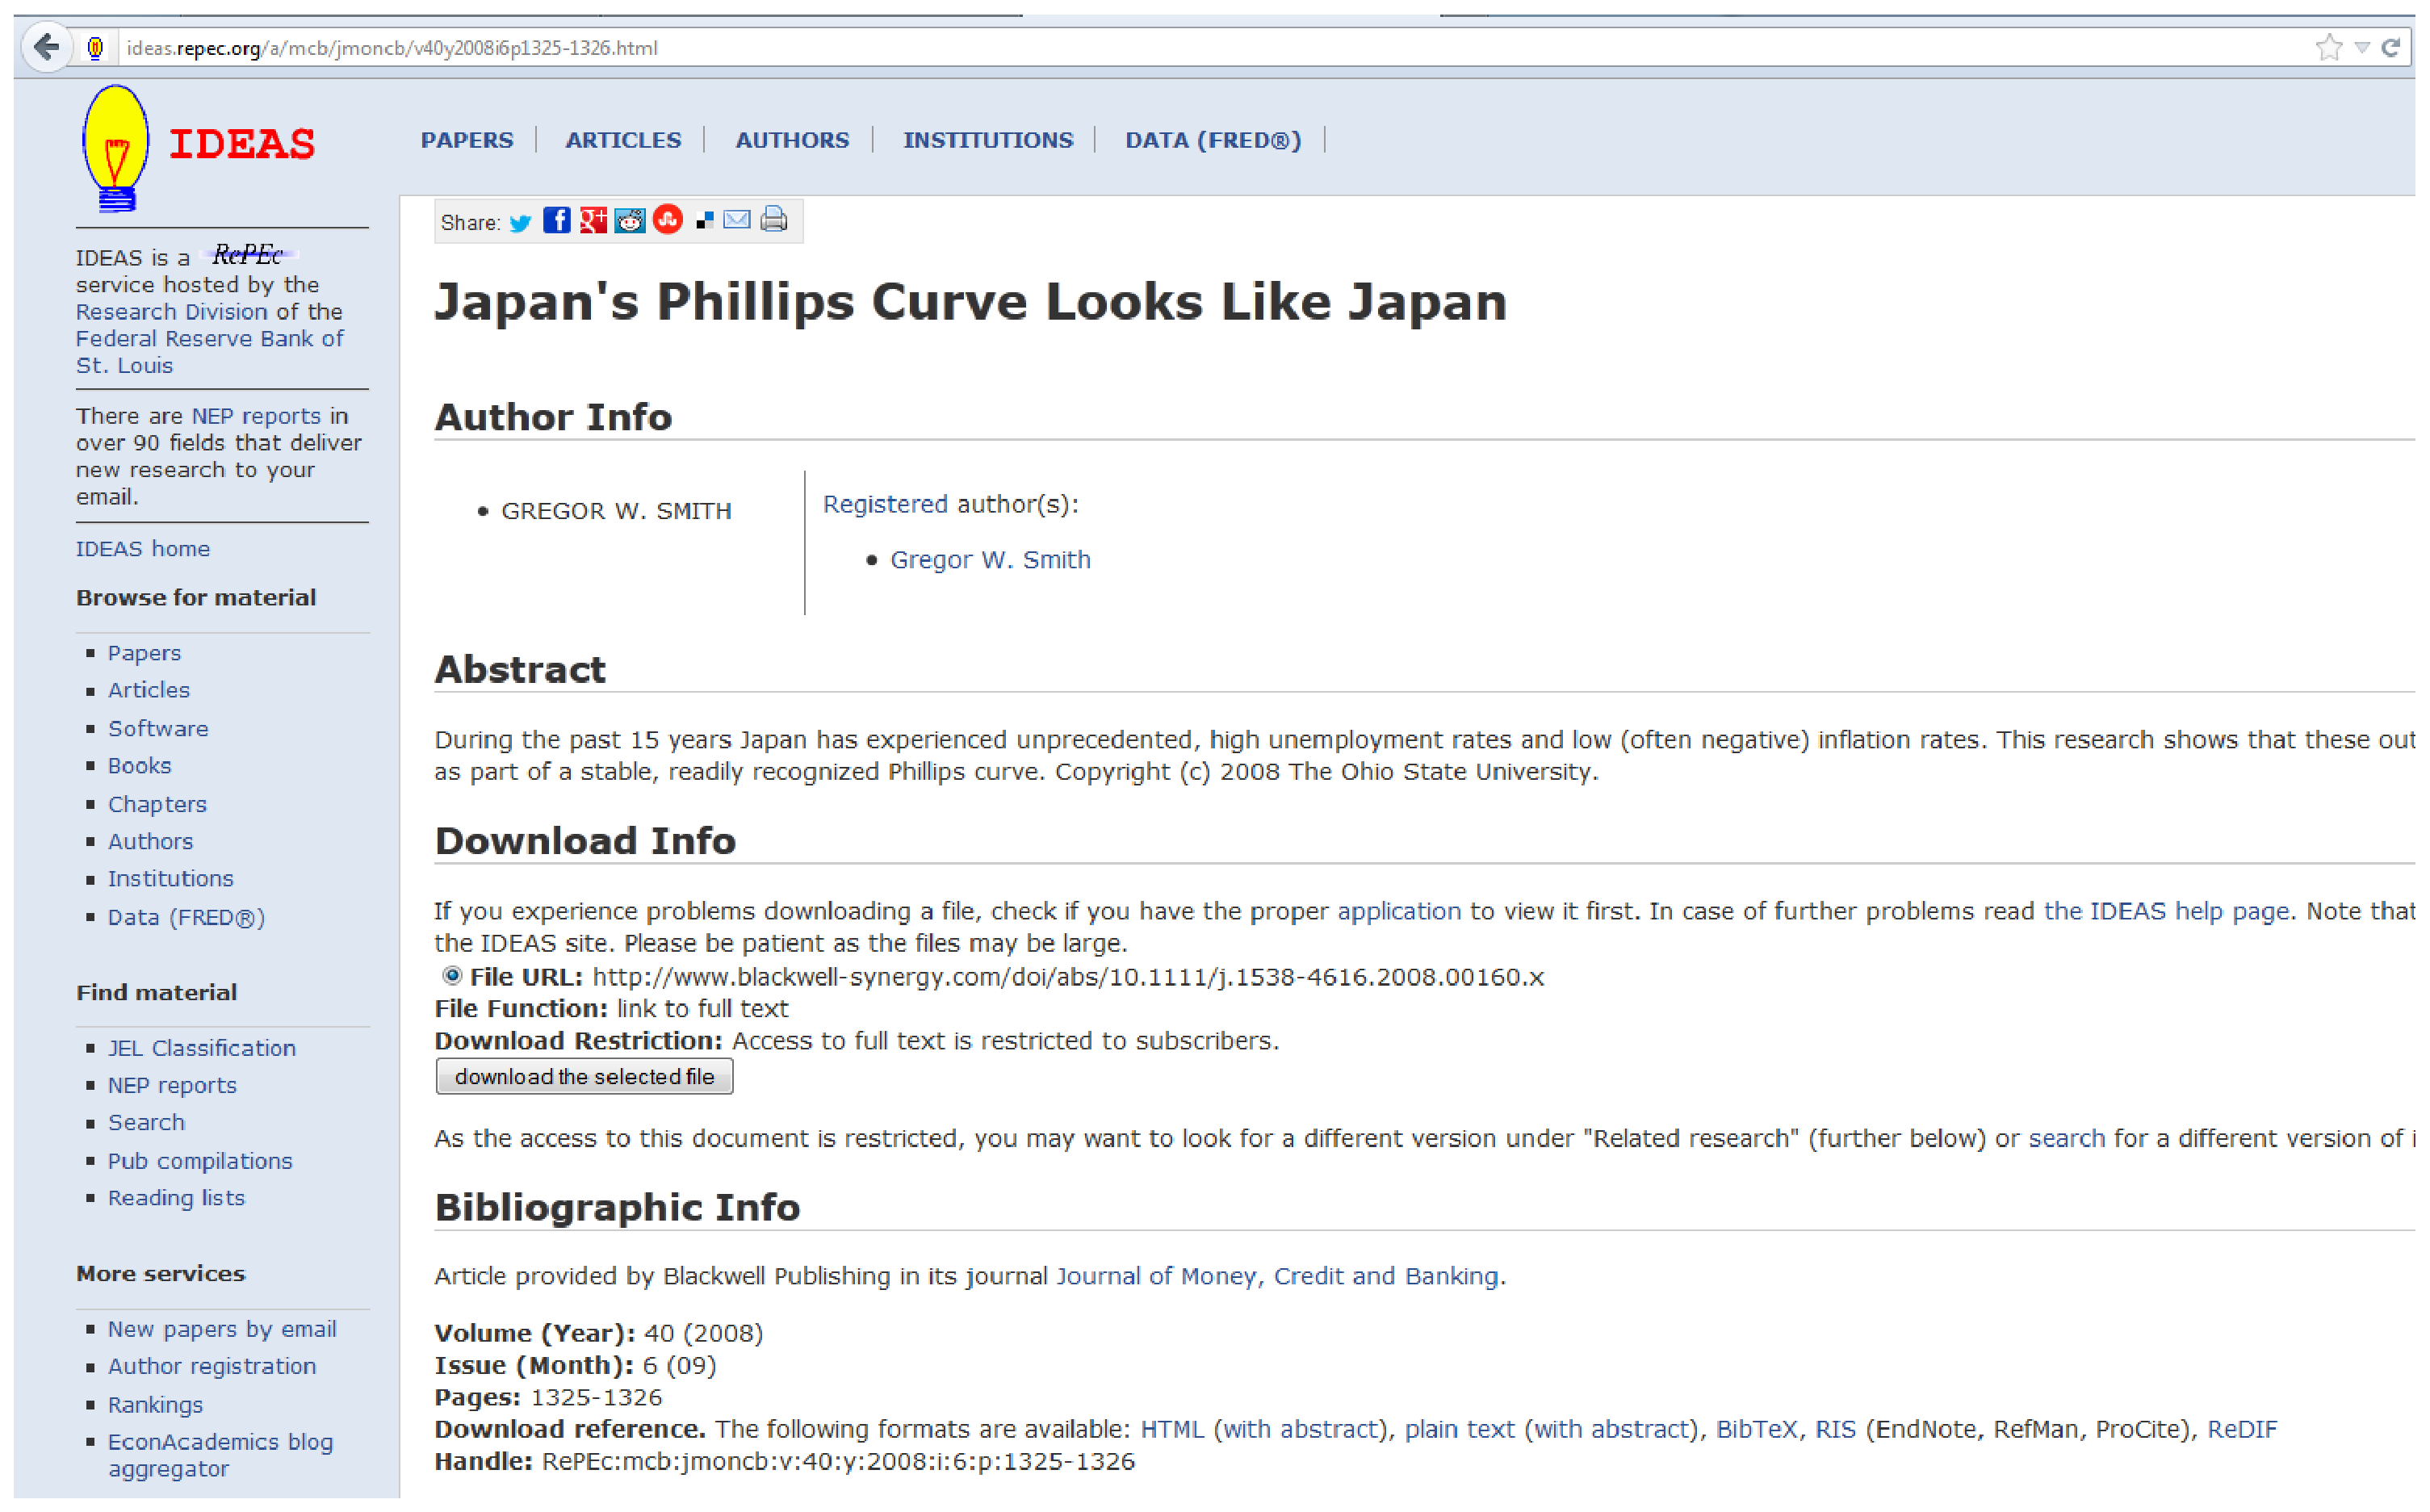
\includegraphics[width=1.0\linewidth]{Ideas}
    \end{minipage}
    \begin{minipage}{0.3\linewidth}
        \begin{enumerate} %enumerate creates a numbered list
            \item This is some text...
            \item This more text
        \end{enumerate}
    \end{minipage}
\end{figure}



\section{References and Citations}
References should be managed using Bib\LaTeX. A good GUI-interface for Windows is JabRef. Download it at \url{http://jabref.sourceforge.net/}. As shown in Figures \ref{fig:Ideas1} and \ref{fig:Ideas2}, you can download the bibliographic information for many economic references from \url{ideas.repec.org} or databases like JSTOR or ScienceDirect. Just copy the Bibtex-key and paste it into Jabref as shown in Figure \ref{fig:jabref}. Try assigning unique and expressive Bibtex-keys, i.e.\ use for example \textit{Smith2006} instead of \textit{Reference1} (or even better \textit{Smith2006Japan}).

\begin{figure}[h!] % h! places the float at this place, use t for top, b for bottom, p for page, can be used in combination to define preference ordering
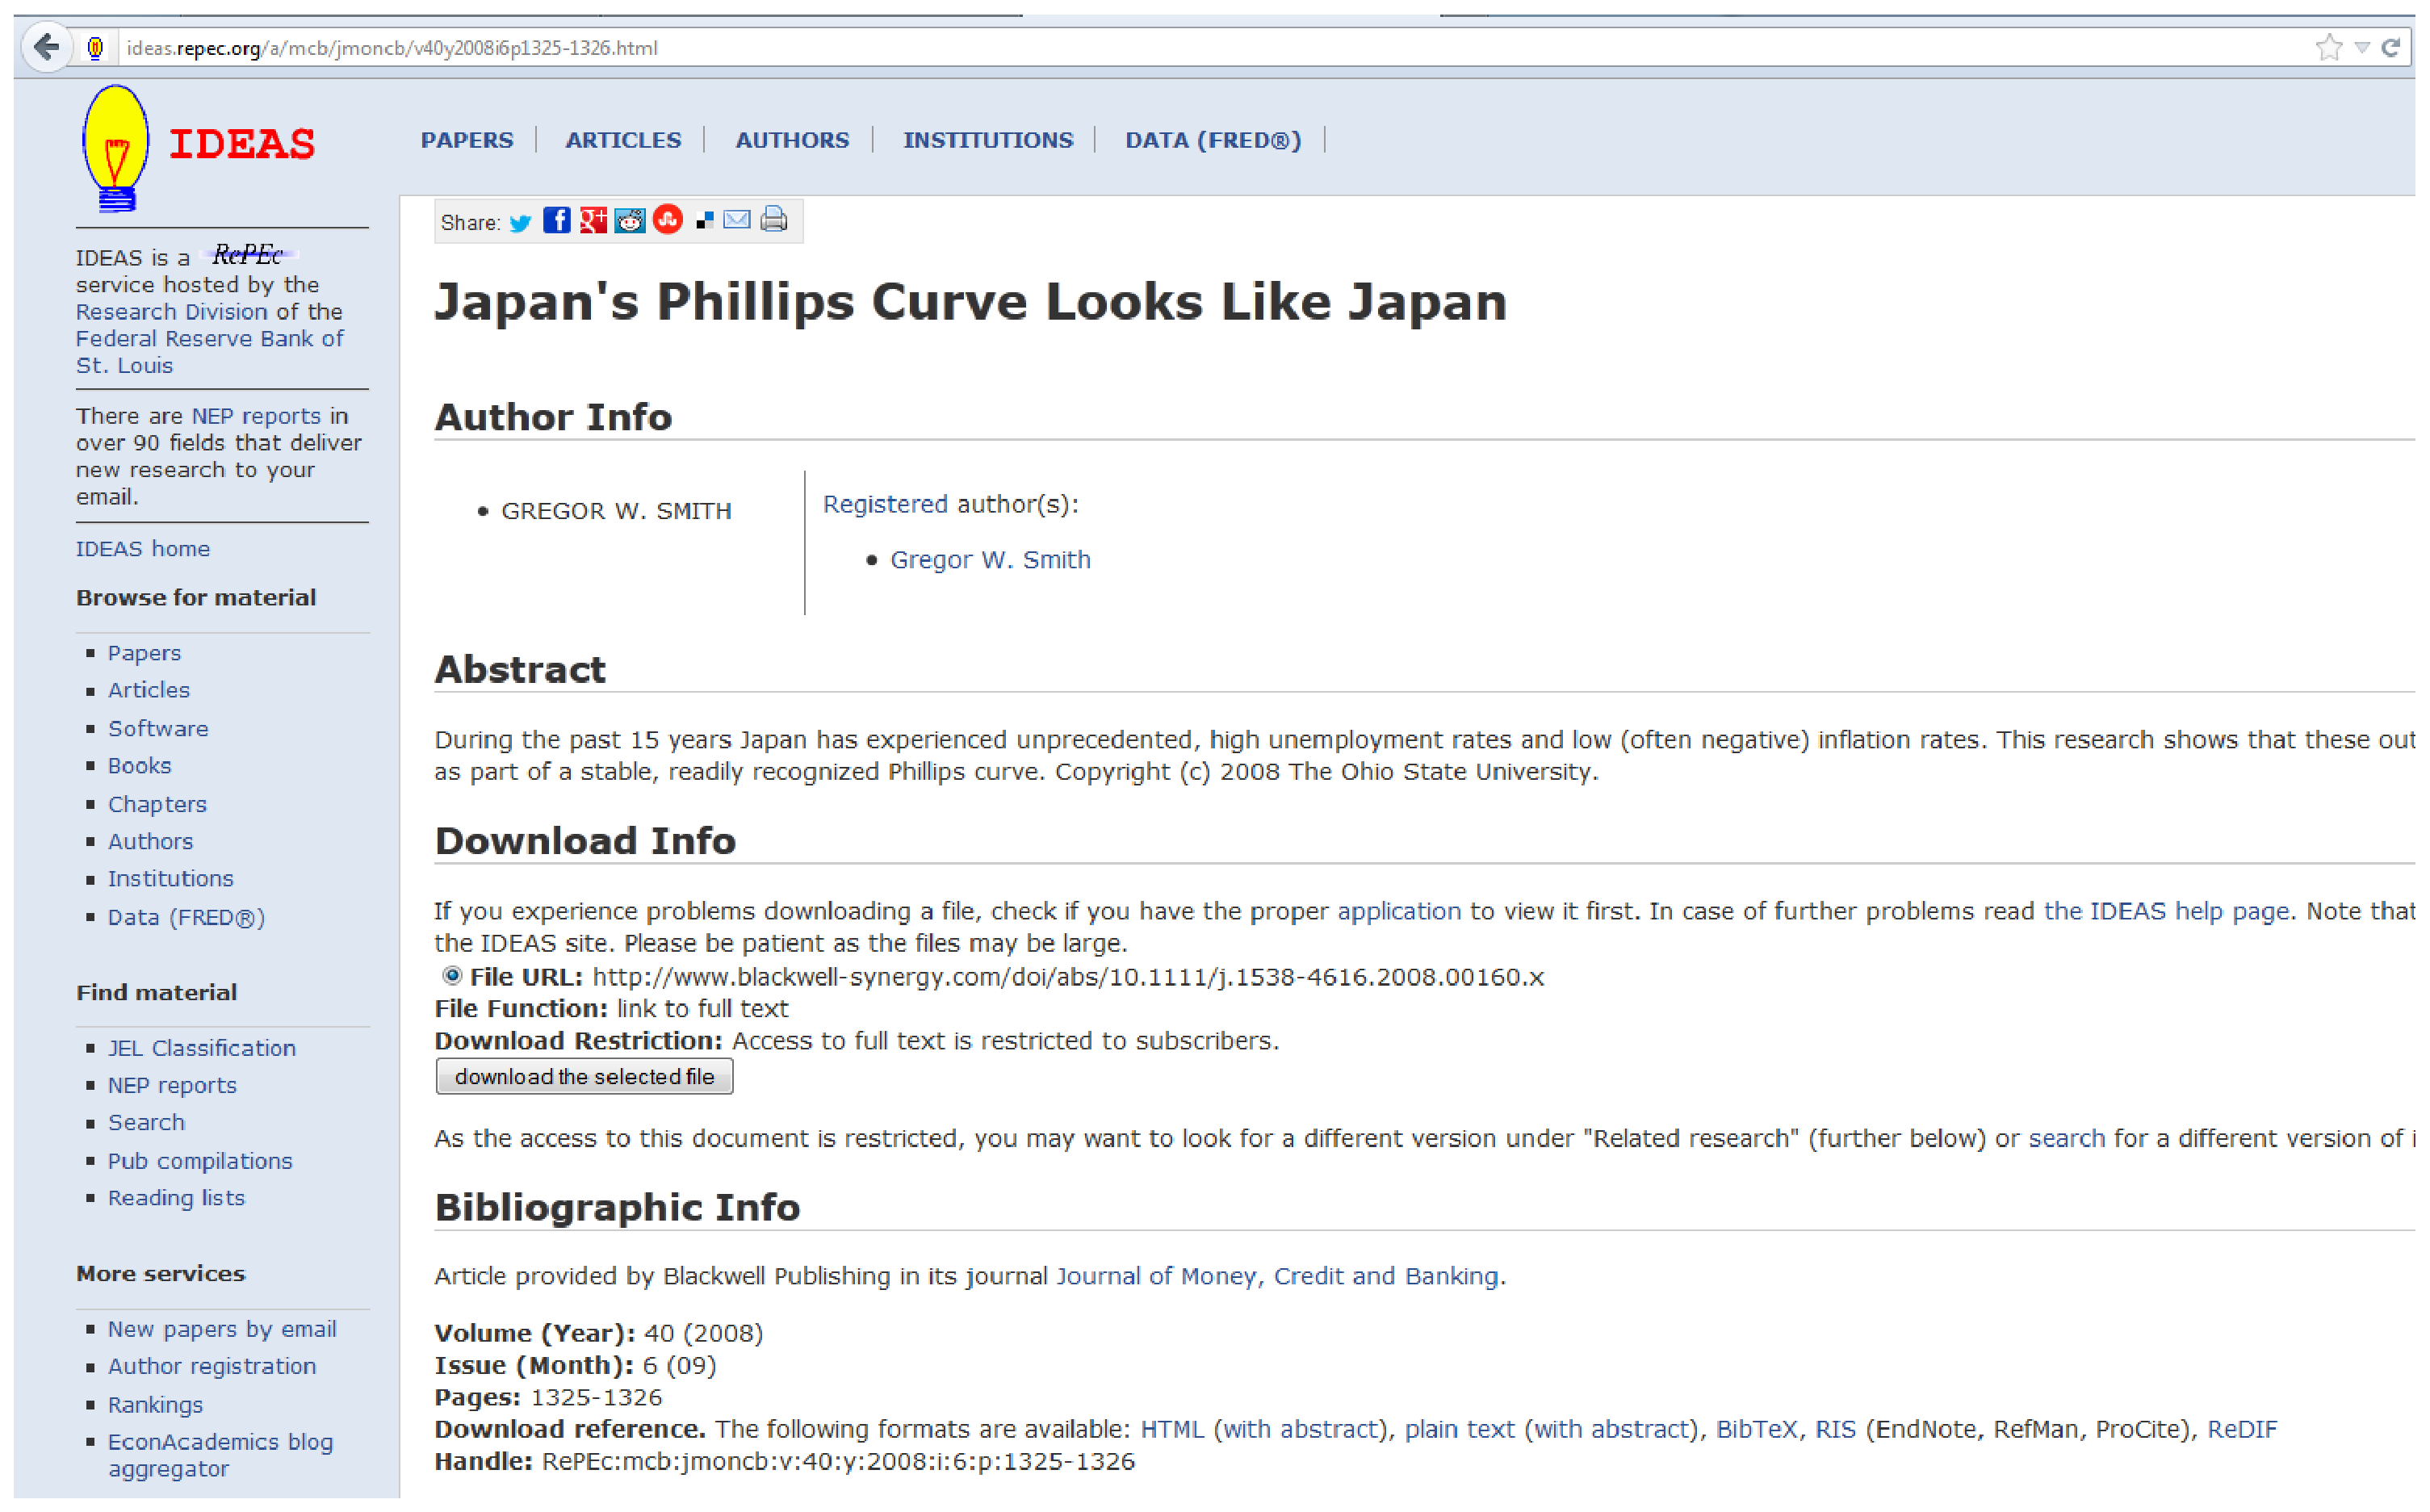
\includegraphics[scale=0.3]{Ideas}  % scales figure to 35%
\caption[Title for List of Figures]{To download the bibliographic information from Repec, klick on \emph{Download reference: Bibtex}}\label{fig:Ideas1} %label, to refer to later
\end{figure}

\begin{figure}[htbp!]
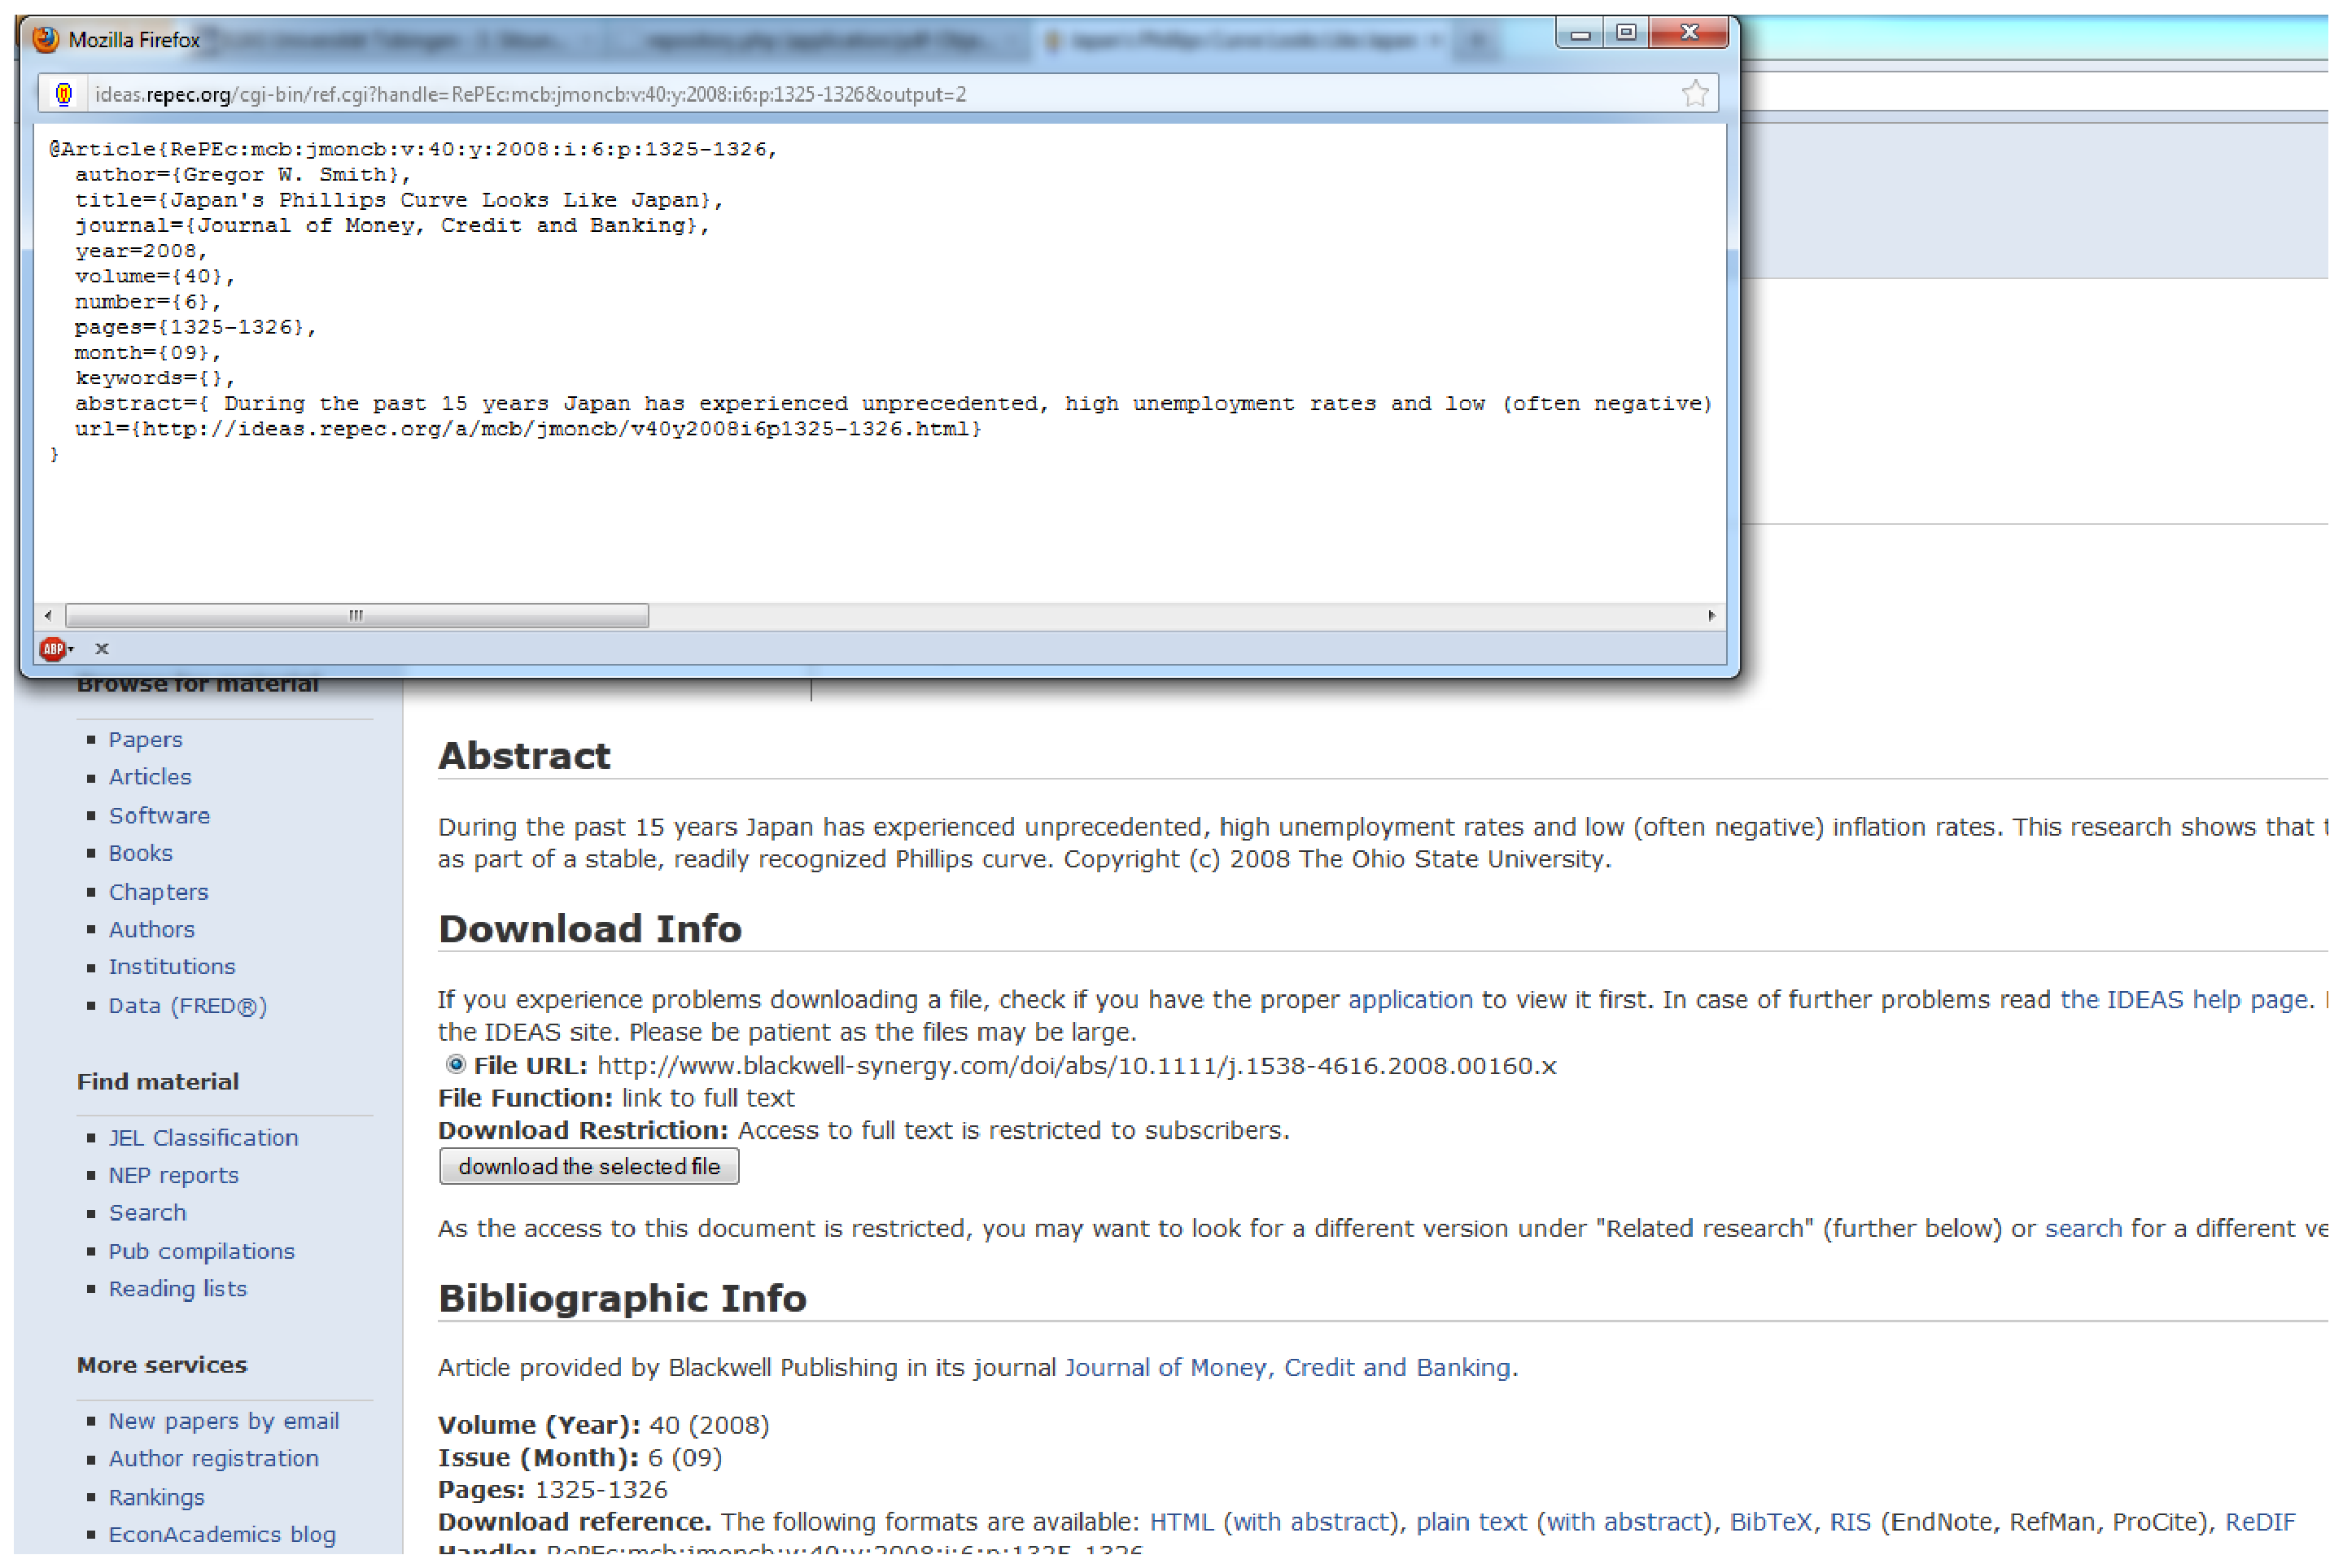
\includegraphics[width=\ScaleIfNeeded]{Ideasbibtex}
\caption[Extracting References from Bibtex]{Copy the text from the window into the memory}\label{fig:Ideas2}
\end{figure}
%
\begin{figure}[htbp!]
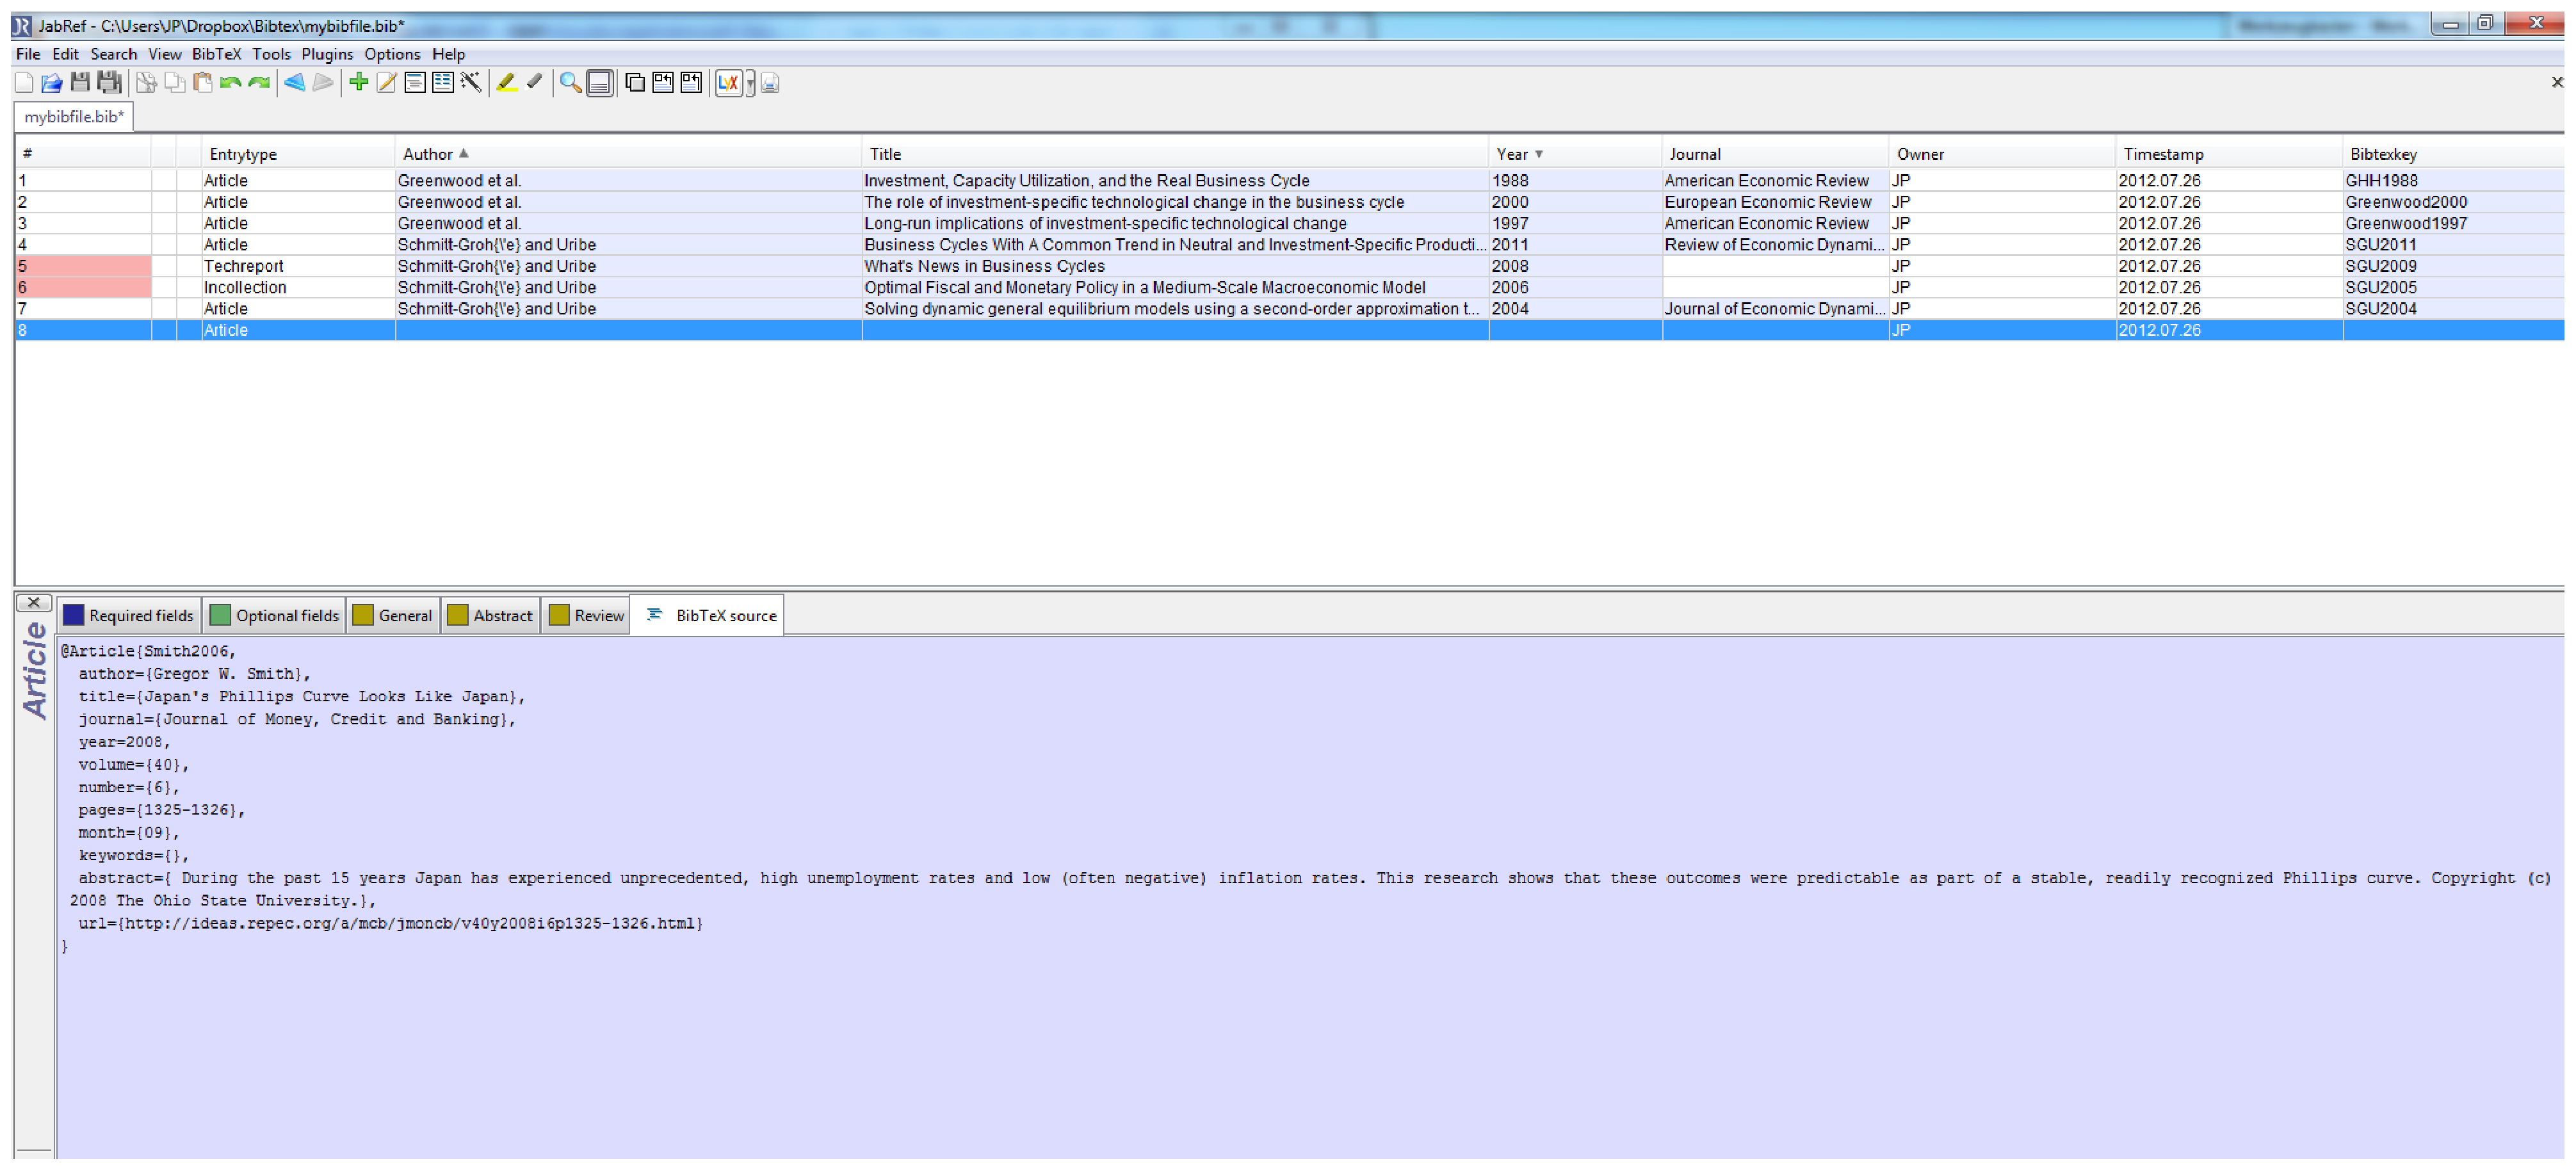
\includegraphics[width=\ScaleIfNeeded]{JabrefAdd}
\caption[Using JabRef]{Klick on the Add-Button (green plus) and paste the copied text to \emph{Bibtex Source}. Do not forget to change the Bibtex-key (the first entry). Here I chose the key \texttt{Smith2006}}\label{fig:jabref}
\end{figure}

Please use inline citations and not citations in footnotes.\interfootnotelinepenalty=5000\footnote{As you can see, footnotes are placed with the \texttt{\textbackslash footnote{}}-command. Sometimes footnotes can become quite long. In this case, \LaTeX\ automatically distributes the footnote over more than one page. Sometimes this automatic setting does not perform the way it should. You can change the behavior by setting \texttt{\textbackslash interfootnotelinepenalty=x}, where $x$ is an integer from $0$ to $10{,}000$, with 100 being the default. When set to $10{,}000$ \LaTeX\ will not split the footnote. The option \texttt{\textbackslash interfootnotelinepenalty=x} can be both set in the preamble to affect all footnotes or in the text immediately before a footnote. In the latter case, it needs to be set back to its default if you want the command to only affect one footnote.} \interfootnotelinepenalty=100  The \texttt{natbib}-compatibility specified in the preamble provides several cite commands.\footnote{For the original Bib\LaTeX-commands that allow for many more options, see \url{http://mirror.ctan.org/macros/latex/contrib/biblatex/doc/biblatex.pdf}.} The command \texttt{\textbackslash citet\{Smith2006\}}, where \textit{Smith2006} is the Bibtex-Key defined in JabRef, cites the reference with the name: \citet{Smith2006}. The command \texttt{\textbackslash citep\{Smith2006\}} cites the reference in parentheses: \citep{Smith2006}. The command \verb|\citep[Prefix][Suffix]\{Smith2006\}| allows for Prefixes and Suffixes in the parentheses: \citep[see e.g.][pp. 1-4]{Smith2006}. More information can be found at \url{ftp://ftp.tex.ac.uk/tex-archive/macros/latex/contrib/natbib/natnotes.pdf}.\\

Bib\LaTeX automatically shortens multiple citations with the same authors, e.g.\ \citep{SGU2004JET,SGU2004,SGU2009,SGU2011} and provides correct referencing with a,b,etc. Moreover, it takes care of different bibliography requirements of articles like \citet{SGU2004} and books like e.g.\ \citet{SGU2005}.\\
The style of the bibliography is controlled using the \verb|bibstyle|-option. The current document uses the JME-style file.\\

For electronic sources like blog-posts \citep[e.g.\ ][]{Krugman2012}, you should use the \texttt{electronic}-entrytype in JabRef. Unfortunately, you must manually add the \texttt{urldate}-field to the Bib\TeX-source as shown in Figure \ref{fig:jabref_urldate} in order to print out the access date. The correct field format is YYYY-MM-DD.

\begin{figure}[htbp!]
\includegraphics[width=\ScaleIfNeeded]{Urldate}
\caption[Adding electronic sources]{For electronic sources, you must manually enter the \texttt{urldate}-field in the Bib\TeX source.}\label{fig:jabref_urldate}
\end{figure}


\section{List of Symbols and Abbreviations}
A List of Symbols and a List of Abbreviations as displayed at the beginning of this document can be created using the \texttt{glossaries} package.\footnote{For more information, see the beginner's guide at \url{http://mirror.ctan.org/macros/latex/contrib/glossaries/glossariesbegin.pdf} and the documentation at \url{http://mirror.ctan.org/macros/latex/contrib/glossaries/glossaries.pdf}.} In case you are using TeXnicCenter, you may have to manually add makeindex to the profile.\footnote{See \url{http://brianhoffmann.de/journal/thesis/2011-08-01/latex-glossaries-with-texniccenter/} or \url{https://tex.stackexchange.com/questions/153323/acronyms-glossaries-not-being-output-in-the-pdf/}.}

\subsection{The \texttt{glossaries} package in the preamble}
The \texttt{glossaries} package is one of the few packages that must be loaded after the \texttt{hyperref}-package. In the current document, I use the standard glossary to list acronyms. In addition to the default glossary, I have defined a second glossary for the List of Symbols, labeled \texttt{symbolslist}, using the command\\
\verb|\newglossary[slg]{symbolslist}{syi}{syg}{List of Symbols}|.\\

After defining the glossaries, you must put \verb|\makeglossaries| to allow for sorting of the glossary entries.\\

To print the List of Abbreviations, put\\
\verb|\printglossary[type=\acronymtype,style=long]|.\footnote{Of course, the style can be changed.}\\
To print the List of Symbols, put\\
\verb|\printglossary[type=symbolslist,style=long,title=List of Symbols]|.

\subsection{Defining the list entries and referencing them}
The entries for the glossaries can either be defined in the preamble or in the main text. For example, the command
\verb|\newglossaryentry{symb:pi}{name={\ensuremath{\pi}}...|, used in the preamble of this document, defines an entry for the glossary \texttt{symbolslist}. However, the symbol \gls{symb:pi} will not appear in the List of Symbols unless you tell \LaTeX\ that you have used it. Usually, you do this by referencing it using the \verb|\gls{}|-command. For example, \verb|\gls{symb:pi}| prints \gls{symb:pi}. This command can also be used inside of equations like this one

\begin{equation}
  \gls{symb:e}^{\gls{symb:i}\gls{symb:pi}}-1=0
\end{equation}

\newacronym{acro:DSGE}{DSGE}{Dynamic Stochastic General Equilibrium} %define new acronym inside of the main document

You can also define symbols or acronyms in the main matter, for example putting \verb|\newacronym{acro:DSGE}{DSGE}{Dynamic Stochastic General Equilibrium}| at the beginning or end of a paragraph where you use the symbol/acronym the first time. Subsequently in the text, you can refer to the acronym using the command \verb|\gls{}|, e.g.\ \verb|\gls{acro:DSGE}|. The first time you use it, \LaTeX\ automatically prints the long version followed by the abbreviation. The second time, only the acronym is printed. For example, \gls{acro:DSGE} will from now on be abbreviated as \gls{acro:DSGE}. Moreover, all symbols/abbreviations referenced with \verb|\gls{}| (or its derived commands) are automatically added to the list of symbols/abbreviations.\\
\textbf{For glossaries to be updated correctly, you usually have to run \LaTeX\ (at least) twice.}\\

If you are not going for the full capabilities of glossaries, you can also just define the symbol or acronym you are using in the preamble and add it to the respective list by putting \verb|\glsadd{}| after the definition as I did with the \verb|\glsadd{OLS}|. In this case, the symbol/acronym will appear in the List of Symbols/Abbrevations even if you did not reference it with \verb|\gls{}|. Hence, this is an quick and dirty way to create such a list. However, this procedure is not advised as you now have to make sure manually that only abbreviations/symbols used at least once in the text appear in the list.



\section{Further Information}

\begin{itemize}
    \item Almost every imaginable \LaTeX-question has been asked before. Just google or search the FAQ at \url{http://www.tex.ac.uk/cgi-bin/texfaq2html?introduction=yes}
    \item There are deadly \LaTeX\ sins you should never commit, see \url{http://queen.elektro.uni-miskolc.hu/~gati/references/latex/latex/l2tabuen.pdf}.
    \item Helpful resources can be found at \url{http://en.wikibooks.org/wiki/LaTeX/}.
    \item For presentations use \LaTeX\ Beamer, see \url{ftp://ftp.fu-berlin.de/tex/CTAN/macros/latex/contrib/beamer/doc/beameruserguide.pdf}.
\end{itemize}

%_________________ End of Main Matter_________________%

\clearpage

%_________________ Reference Section _______________%

\phantomsection                                   % allows for correct link to Table of Contents
\addcontentsline{toc}{section}{References}        % Adds the line "References" to Table of contents
\onehalfspacing


\printbibliography % print the bibliography using BibLaTex


%% alternative using BibTeX
%\bibliographystyle{econometrica}                  % sets the style for the Bibliography
%\bibliography{mybibfile}                         % Uses the Bibtex-file mybibfile.bib


\clearpage
%_________________ Space for Supplementary Material _______________%
\appendix
\numberwithin{equation}{section} %restarts equation numbering with 1 and adds the appendix in front
\numberwithin{table}{section} %same for Tables
\numberwithin{figure}{section} %and for Figures

\section{Appendix 1}

Some Information relegated to the appendix.
\begin{equation}
    MV=PQ
\end{equation}

\pagebreak

\section{Supplementary Tables}




\begin{table}[h!] % h! places the float at this place, use t for top or b for bottom
\caption{Title of the table}
\label{tab:SuppTable1}
\centering
 \begin{tabular}{lcr}
   Another & small & table\\
\toprule
   left aligned & centered & right aligned \\
   \multicolumn{2}{c}{Text over two columns} & third column \\
\bottomrule
\end{tabular}
\caption*{\footnotesize{\emph{Notes:} Add the description here}}
\end{table}

\clearpage

\section{Eidesstattliche Versicherung/Affidavit}

Ich versichere, dass ich die vorliegende Arbeit ohne Hilfe Dritter und ohne Benutzung anderer
als der angegebenen Quellen und Hilfsmittel angefertigt und die den benutzten Quellen
wörtlich oder inhaltlich entnommenen Stellen als solche kenntlich gemacht habe. Diese Arbeit
hat in gleicher oder ähnlicher Form noch keiner Prüfungsbehörde vorgelegen.\\
Ich bin damit einverstanden, dass meine Arbeit zum Zwecke eines Plagiatsabgleichs in
elektronischer Form anonymisiert versendet und gespeichert werden kann.\\

\vspace{1cm}

I affirm that this Bachelor thesis was written by myself without any unauthorised third-party
support. All used references and resources are clearly indicated. All quotes and citations are
properly referenced. This thesis was never presented in the past in the same or similar form to
any examination board.\\
I agree that my thesis may be subject to electronic plagiarism check. For this purpose an
anonymous copy may be distributed and uploaded to servers within and outside the University
of Mannheim.

\vspace{3cm}
\makebox[\textwidth]{\hrulefill \hspace{3cm} \hrulefill}

Ort, Datum/Place, Date \hfill Unterschrift/Signature



\end{document}
